\documentclass{standalone}
\input{feynman_settings}

\usetikzlibrary{patterns, decorations.markings, snakes, calc, decorations.pathreplacing, decorations}

\usepackage{relsize} %larger math symbols

\begin{document}

%actual code
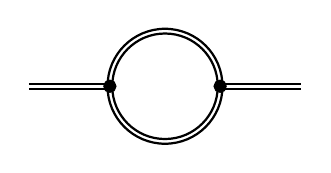
\begin{tikzpicture}

%External Lines
\draw[thick] (0,0.03) to (1,0.03); 
\draw[thick] (0,-0.03) to (1,-0.03); 
\draw[thick] (2.46,0.03) to (3.46,0.03); 
\draw[thick] (2.46,-0.03) to (3.46,-0.03); 
%Loop 1
\draw[thick] (1.73,0)  circle(0.73);
\draw[thick] (1.73,0)  circle(0.67);


%Vertices
\draw[thick, fill = black] (1.03,0) circle (0.07);
\draw[thick, fill = black] (2.43,0) circle (0.07);
%\node [draw, fill = white, circle, cross, minimum width= 0.1 cm] at (0,0.7){}; 
\end{tikzpicture}
\raisebox{4ex}{$\quad \mathlarger{+} \ $ }
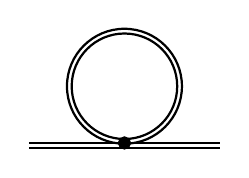
\begin{tikzpicture}

%External Lines
\draw[thick] (0,-0.72) to (2.43,-0.72); 
\draw[thick] (0,-0.78) to (2.43,-0.78); 

%Loop 2
\draw[thick] (1.215,0)  circle(0.73);
\draw[thick] (1.215,0)  circle(0.67);

%Vertex
\draw[thick, fill = black] (1.215,-0.72) circle (0.07);
\end{tikzpicture}
\raisebox{4ex}{$\quad \mathlarger{\propto} \quad G \ (p^2)^2 $ }

\end{document}